\section{Motivation}
\label{sec:motivation}
In diesem Versuch wird ein Helium-Neon-Laser in Betrieb genommen und in seinen Eigenschaften vermessen.
Verschiedene Laser sind in vielfältigen wissenschaftlichen und alltäglichen Anwendungen in Betrieb.
Der wissenschaftliche Betrieb reicht von Spektroskopie und optischem Pumpen bis hin zu
Detektionslasern für Gravitationswellen.
Im nichtwissenschaftlichen Bereich werden Laser sehr bekannt in Laserpointern,
aber auch in Streckenmessungen oder Computermäusen verwendet.
Die Messaufgaben dieses Versuches decken die grundlegenden Funktionsweisen
und Eigenschaften eines Lasers ab.

\section{Theorie}
\label{sec:theorie}
Ein Laser besteht aus drei Grundkomponenten, dem aktiven Medium, der Energiepumpe und dem Resonator \cite{demtroeder}.

\subsection{Laser-Aufbau}
Die Energiepumpe kann in vielerlei Varianten auftreten.
Häufig ist es eine Blitzlampe oder eine Elektrodenstrahlröhre.
In dem verwendeten Aufbau ist es eine Elektrodenstrahlröhre.

Diese Elektronen regen im aktiven Medium die Elektronen der Atome an.
Es erfolgt eine Anregung vom Grundniveau $\ket{i}$ ins Niveau $\ket{k}$.
Ist das Niveau $\ket{k}$ gesättigt, kommt es zu einer stimulierten Emission.
Hierbei fällt ein Elektron von $\ket{k}$ nach $\ket{i}$.
Es kommt zur Emission eines Photons mit der Frequenz
\begin{equation}
  ν = \frac{E_k-E_i}{\hbar}\,.
\end{equation}

Dieses Photon hat eine zufällige Winkelverteilung.
Um die Photonen zu konzentrieren wird um das aktive Medium ein Resonator gebaut.
In diesem Resonator schwingen die Photonen zwischen den Resonatorgrenzen
durch das aktive Medium hindurch.
Beim Durchgang durch das Medium werden weitere Elektronen zum Sprung ins untere Niveau $\ket{i}$.
Bei einem Drchgang kommt es hier zu einer Kettenreaktion, da die neu entsandten Photonen ebenfalls
Emissionen anregen.
Die frei werdenden Stellen im Niveau $\ket{k}$ werden durch die Anregung mit der Enrgiepumpe
wieder gefüllt, dieser Vorgang wird \textit{pumpen} genannt.
\\~\\
Im Experiment wird ein offener Resonator verwendet.
Hierbei handelt es sich um zwei Spiegel.
Diese müssen ein hohes Reflexionsvermögen haben um die Verluste durch Absorption zu minimieren.
Zudem muss einer der Spiegel eine nicht verschwindende Transmissionwahrscheinlichkeit besitzen,
um den Strahl auskoppeln zu können.
Für die Spiegel wird in Verbindung mit der Resonatorlänge $L$ der Stabilitätsparameter
\begin{align}
  g_i &= 1 - \frac{L}{r_i}\,. \label{eqn:stabi}
  \intertext{Das Produkt $g_1\cdot g_2$ gibt an, ob das System stabil ist.
    Es gelten die Bedingungen für Stabilität}
  0 &< g_1\cdot g_2 < 1
  \intertext{oder}
  0 &= g_1 = g_2\,.
\end{align}
In Abbildung \ref{fig:vorbereitung} sind die Kurven für die Kombinationen der zwei Linsen
gegen die Resonatorlänge aufgetragen.

\begin{figure}
  \centering
  \includegraphics[width=0.8\textwidth]{build/vorbereitung.pdf}
  \caption{Abhängigkeit des Stabilitätsparameters $g_1\cdot g_2$ von der\\
      Resonatorlänge $L$ für verschiedene Kombinationen an Spiegeln.}
  \label{fig:vorbereitung}
\end{figure}

An den Enden des Gasröhre in der das aktive Medium, hier das $\ce{HeNe}$-Gas,
ist an jedem Ende ein Brewsterfenster verbaut.
Diese sorgen dafür, dass das Laserlicht linear polarisiert ist.

\subsection{Transversale Elektrische Moden}
Im Laserstrahl bilden sich verschiedene Moden aus, unteranderem \textbf{T}ransversale \textbf{E}lektrische \textbf{M}oden.
Gemessen werden können $\text{TEM}_{00}$ und $\text{TEM}_{10}$.
Die Intensitätsverteilung ist in Abbildung \ref{fig:tem-theorie} gezeigt.
\begin{figure}
  \centering
  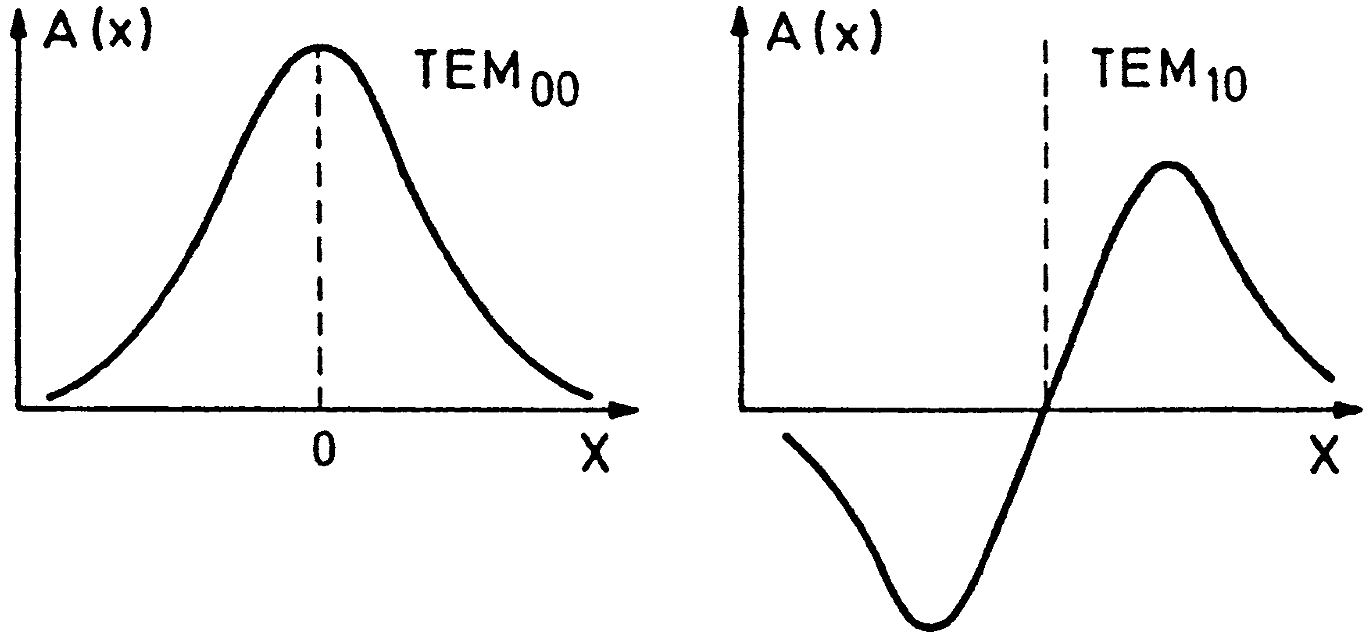
\includegraphics[width=0.8\textwidth]{images/tem-theorie.png}
  \caption{Visualisierung von $\text{TEM}_{00}\:\&\:\text{TEM}_{10}$. \cite{demtroeder}}
  \label{fig:tem-theorie}
\end{figure}

\FloatBarrier
\subsection{Beugungsspektrum}
Fällt ein kohärenter Lichtstrahl durch ein Gitter,
entsteht dahinter ein Beugungsmuster aufgrund der Interferenz der am Gitter entstehenden
Kugelwellen. Wird in einer Entfernung $a$ zum Gitter ein Schirm orthogonal zur Strahlrichtung
sind Maxima und Minima zu erkennen.
Daraus kann die Wellenlänge $λ$ mit der Formel
\begin{equation}
  λ = \frac{b\cdot d_k}{k\cdot\sqrt{a^2+d_k^2}}
  \label{eqn:gitter}
\end{equation}
bestimmt werden \cite{gitter}.
Es gelten die Bezeichnungen
\begin{align*}
  b &: \text{inverse Gitterkonstante} \\
  d_k &: \text{Abstand des $k$-ten Maximus vom 0ten Maximum} \\
  k &: \text{Ordnung des Maximus} \\
  a &: \text{Abstand zwischen Gitter und Schirm.}
\end{align*}
